\mysection{Prblem Set 2.5}

\begin{description}
  \setlength{\parskip}{0cm} % 段落間
  \setlength{\itemsep}{0cm} % 項目間
  \item[1 回答] Value順にソートし、貪欲法を適用したItemを表\ref{tb1}に示す。

  \begin{table}[ht]
  \centering
  \caption{Value順ソート後に貪欲法を適用したItem}
  \begin{tabular}[t]{cccccc}
  \toprule
  Item&&D&E&B&I\\
  \midrule
  Items packed&$\phi$&\{D\}&\{D, E\}&\{D, E\}&\{D, E, B, I\}\\
  Total weight&0&22&40&40&48\\
  Total Value&0&10&19&19&26\\
  \bottomrule
  \end{tabular}
  \label{tb1}
  \end{table}%
  次にweightあたりのvalueの値が大きい順になるように貪欲法を適用したItemを表\ref{tb2}に示す。
  
  \begin{table}[ht]
  \centering
  \caption{weightあたりのvalueの値が大きい順になるように貪欲法を適用したItem}
  \scalebox{.55}{
  \begin{tabular}[t]{cccccccccccc}
    \toprule
    Item&&A&G&I&H&B&C&E&D&J&F\\
    \midrule
    Items packed&$\phi$&\{A\}&\{A, G\}&\{A, G, I\}&\{A, G, I, H\}&\{A, G, I, H, B\}&\{A, G, I, H, B, C\}&\{A, G, I, H, B, C\}&\{A, G, I, H, B, C\}&\{A, G, I, H, B, C, J\}&\{A, G, I, H, B, C, J\}\\
    Total weight&0&3&6&14&20&32&37&37&37&45&45\\
    Total Value&0&6&10&17&22&30&33&33&33&35&35\\
    \bottomrule
    \label{tb2}
    \end{tabular}
    }
    \end{table}%
  \end{description}

\mysection{Problem Set 3.1}

\begin{description}
  \setlength{\parskip}{0cm} % 段落間
  \setlength{\itemsep}{0cm} % 項目間
  \item[4 回答] $p=q+1$を満たす木でないグラフの一例を図\ref{g1}に示す。
  \begin{figure}[h]
    \begin{center}
      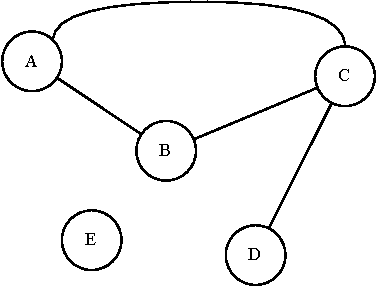
\includegraphics[width=.45\linewidth]{img/graph1.pdf}
    \end{center}
    \caption{$p=q+1$を満たす木でないグラフの一例}
    \label{g1}
  \end{figure}
\end{description}